\documentclass{article}
\usepackage{amsmath}
\usepackage[utf8]{inputenc}
\usepackage{graphicx} % Comandos para manejar imágenes
\graphicspath{ {./images/} } % Carpeta de imágenes
\usepackage[table,xcdraw]{xcolor}
\setlength{\parskip}{2mm} % Espaciado

\usepackage[utf8]{inputenc}
\usepackage{geometry}
    \geometry{left=3cm,right=2cm,top=2cm,bottom=2cm}
%
\usepackage[spanish]{babel}
%
\usepackage[fixlanguage]{babelbib}
    \bibliographystyle{babunsrt}
%

\usepackage{floatrow}
\floatsetup[table]{style=plaintop}

\usepackage{url}

\usepackage[top=2cm, bottom=2.5cm, right=3 cm, left=3 cm]{geometry} % margenes

\usepackage{parskip} % Sangria

\title{Creencias personales en el consumo de bienes y servicios energéticos}
\author{Cristóbal Galleguillos Ketterer$^{1}$\\
\small{$^{1}$Industrial PhD Program}\\
\small{Pontificia Universidad Católica de Valparaíso}\\
\small{cristobal.galleguillos@pucv.cl}
}
\date{\small{\today}}

\begin{document}

\maketitle

\section{Resumen}

Se propone el estudio de las decisiones económicas de los consumidores, considerando en algunos de los casos sus acciones económicas no consideran aspectos racionales, que sean derivados de su capacidad adquisitiva y de sus creencias personales.

En el tema de las creencias personales hemos elegido considerar el consumo de bienes y servicios intensivos en el uso de energía, en su más amplio espectro.

Se propone que el análisis sea holístico e incorpore a su vez conceptualizaciones energéticas, tales como el concepto de entropía, este punto de vista, conocido como bio-economía, se complementa con el estudio del comportamiento de los consumidores y la economía energética propiamente tal.

Se intentará desarrollar un análisis que permita explicar cómo la demanda final de estos consumidores irracionales, afecta los patrones de consumo de la matriz energética para un determinado sector de la economía del que se dispongan datos.

\section{Palabras clave}

Las palabras clave de este estudio son:

\begin{itemize}
    \item Energía
    \item Economía
    \item Teoría de Juegos
    \item Comportamiento del consumidor
    \item Bio-Economía
    
\end{itemize}

\section{Discusión bibliográfica}
 
Para el desarrollo de este trabajo de investigación hemos considerado el estudio de diversas líneas de investigación, que consideraron en primera instancia aspectos clásicos de la economía energética, como el uso intensivo de carbón en la generación de electricidad y los diversos impactos ecológicos y sociales.

Con el desarrollo de la investigación bibliográfico, se decidió poner el foco en la demanda, considerando, que si bien para el consumidor final es ciega la matriz de consumo, el espectro de uso de energía es mucho más amplio que un mero consumo de electricidad, para ello se recurrió a la bibliografía asociado a la economía del comportamiento.

Finalmente, mediante una exploración de las interacciones entre la energía y la economía se llegó al concepto de la bio-economía, mediante el cual se integran ambos conceptualizaciones y se adapta la segunda ley de la termodinámica al estudio de la economía, lo que puede tener interpretaciones interesantes dentro del marco del estudio del comportamiento del consumidor.

El estudio se inició con los aspectos asociados a la emisión de gases efecto invernadero y la eficiencia energética para China \cite{li_metafroniter_2015}, a partir de este texto de siguió explorando con el análisis de las tarifas de gas \cite{gong_evaluating_2016}, mediante economía computacional, este aspecto aún resulta interesante en la potencial investigación que se desarrolle considerando que se encuentre una cantidad de datos significativa.

Al querer expandir el modelo, a los aspectos de la demanda, se comenzó con un análisis de textos clásicos de teoría de juegos \cite{osborne_course_1994}, dentro de este estudio bibliográfico se pudo llegar a trabajos que estudian comportamientos de equilibrio competitivo donde los consumidores son incapaces de adaptar sus decisiones a los precios \cite{gul_coarse_2017}.

Para finalizar se revisó un análisis de la literatura \cite{maneschi_nicholas_2020} acerca de la bio-economía donde se indaga críticamente a paradigma de la racionalidad del consumidos.

Se presenta un \textit{core} disímil en apariencia pero que puede permitir el desarrollo de un análisis general del fenómeno del consumo de bienes intensivos de la energía.

\section{Marco Teórico}

La primera referencia que tenemos de la energía es aquella asociada el consumo de electricidad, sin embargo, el fenómeno energético está presente en todos los patrones de consumo de la sociedad, desde un alimento, el uso de combustibles o la huella energética de un equipo de telefonía móvil.

En este sentido, el marco teórico de este trabajo (ver \ref{mt}), tal y como se discutió en la discusión bibliográfica se basa en tres aspectos:

\begin{figure}[H]
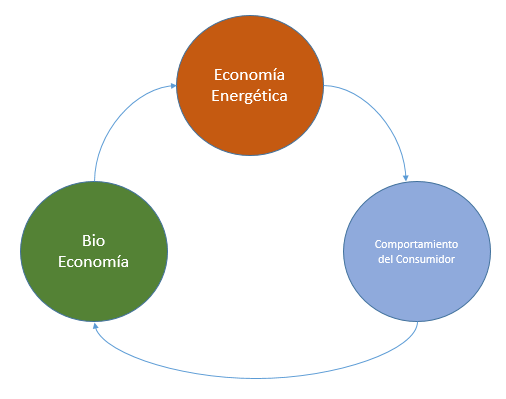
\includegraphics[scale=0.7]{biblio/MarcoTeorico.png}
\centering
\caption{Marco Teórico}
\label{mt}
\end{figure}

 \section{Análisis Bibliográfico}

Para el análisis bibliográfico se buscó la literatura relacionada en la base de datos de Scopus, para mediante la biblioteca Bibliometrix de RStudio realizar un análisis de esta, a partir de la búsqueda de las palabras clave.

La imagen \ref{pc} presenta la producción científica en estas materias, de la revisión del gráfico resulta evidente el interés creciente en estas temáticas.

\begin{figure}[H]
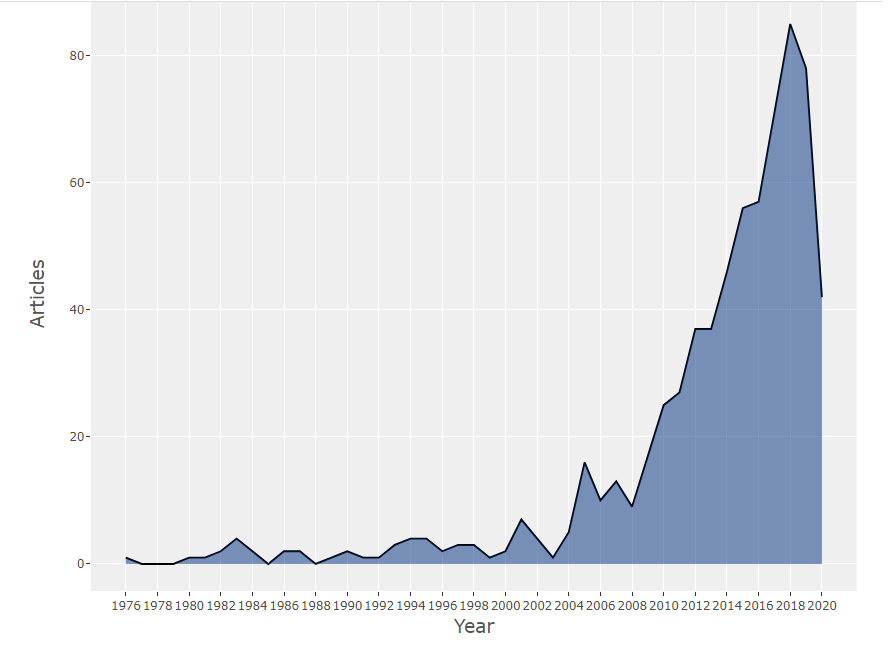
\includegraphics[scale=0.45]{biblio/ProduccionCientifica.png}
\centering
\caption{Producción científica anualizada}
\label{pc}
\end{figure}

Una revisión \ref{mp} a la nube de palabras permite revisar otras temáticas conexas al estudio de interés y ver su peso relativo.

\begin{figure}[H]
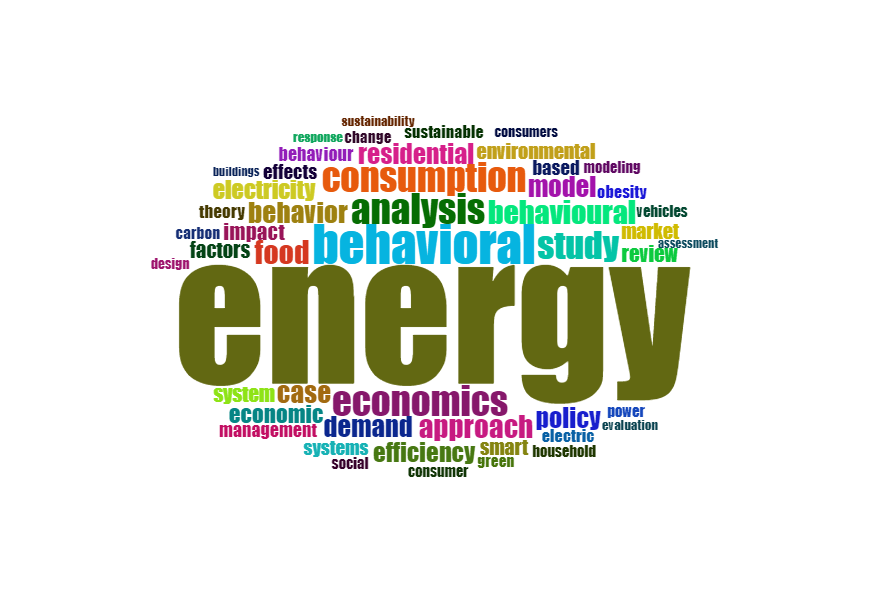
\includegraphics[scale=0.45]{biblio/Mapa de palabras.png}
\centering
\caption{Nube de Palabras}
\label{mp}
\end{figure}

Una visión similar se puede obtener de \ref{tm}

\begin{figure}[H]
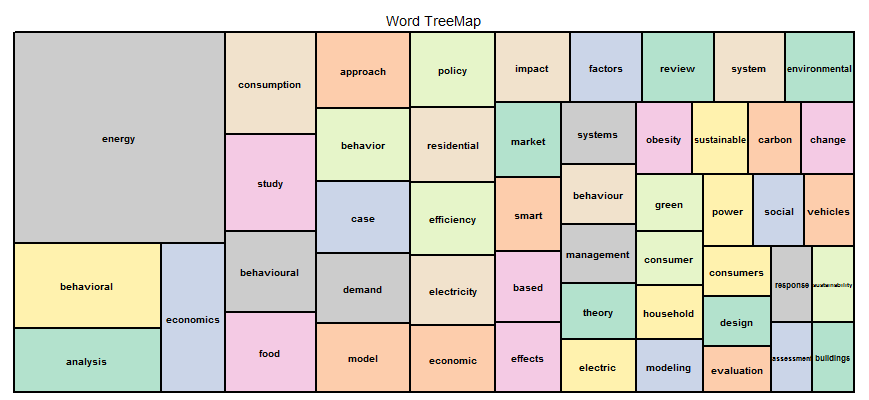
\includegraphics[scale=0.45]{biblio/ThreeMap.png}
\centering
\caption{Three Map}
\label{tm}
\end{figure}

Para entender la evolución del estudio de la Bio-Economía \cite{georgescu-roegen_1972_1976}, utilizamos la aplicación web \textit{Conected Papers} esta nos permite apreciar el margen de tiempo de influencia de una publicación, en este caso 1968 al 2012 y su influencia. 

\begin{figure}[H]
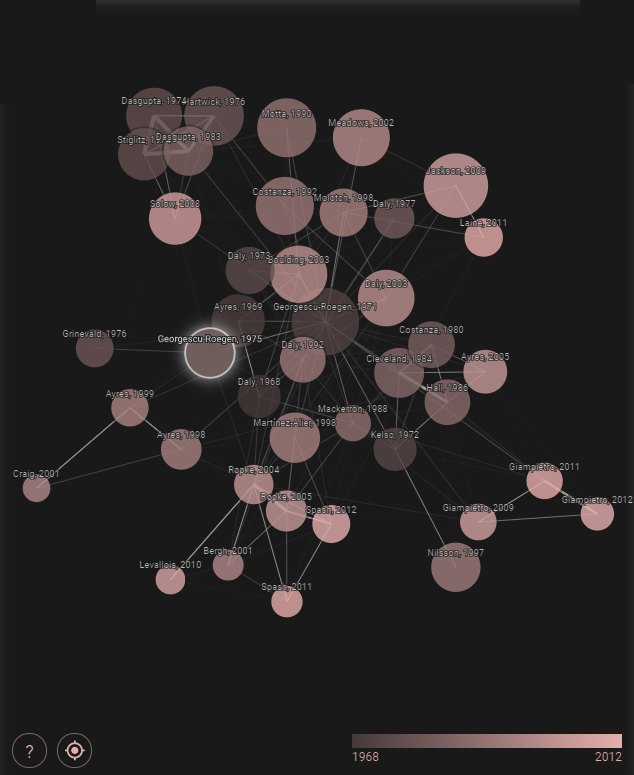
\includegraphics[scale=0.6]{biblio/Paper conectados.png}
\centering
\caption{Bio-economía}
\label{pc1}
\end{figure}

Del mismo modo se analizó un articulo del area del comportamiento del consumidor\cite{gul_coarse_2017}.

\begin{figure}[H]
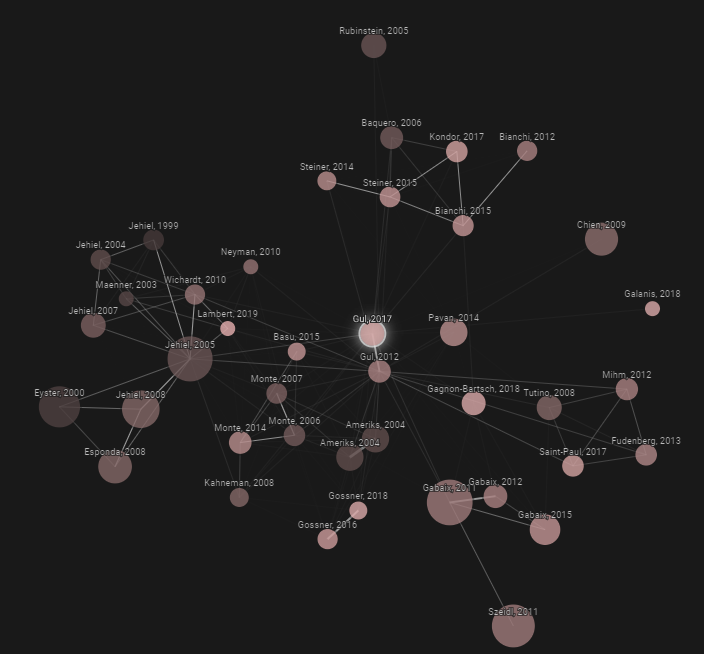
\includegraphics[scale=0.6]{biblio/Paper conectados 2.png}
\centering
\caption{Comportamiento del consumidor}
\label{pc2}
\end{figure}


\nocite{*}
    \bibliography{biblio/seudo}

\end{document}
